\documentclass[10pt]{beamer}
\usetheme{AnnArbor}

\tolerance 99999
\hbadness 99999

\usepackage{amsmath,amsthm,amssymb,color,latexsym}
\usepackage{cancel}
\usepackage{graphicx}
\graphicspath{{images/}}
\setbeamertemplate{items}[ball]

\setbeamertemplate{footnote}{%
  \parindent 1em\noindent%
  \raggedright
  \insertfootnotetext\par%
}
\newcommand{\la}{\mathcal{L}}
\newcommand{\ma}{\mathcal{M}}
\newcommand{\ua}{\mathcal{U}}

\hypersetup{
  colorlinks,
  allcolors=.,
  urlcolor=blue,
}


\newenvironment{points}{\vspace{0.3cm} \begin{enumerate}[label={(\alph*)}]}{\end{enumerate} \vspace{0.2cm}}

\title[J-JEPA]{Jet-Based Joint Embedding Predictive Architecture (J-JEPA)}
\subtitle{CCNSB Seminar}

\author[Abhiram Tilak]
{\textbf{Abhiram Tilak}}

\institute[IIITH]
{
	\textit{\tiny{CND Dual Degree}} \\
	\textit{IIIT Hyderabad}
}


\let\olditemize\itemize
\let\endolditemize\enditemize
\renewenvironment{itemize}{
  \olditemize[<+->] % Apply <+-> to all items
}{\endolditemize}

\date{\today}

\begin{document}

\begin{frame}
	\titlepage
\end{frame}

\begin{frame}
\frametitle{Table of Contents}
\tableofcontents
\end{frame}

\section{Introduction}

\begin{frame}{Introduction}{About the Paper}
  This paper was showcased as a part of workshop ML4JETS2024 held on
  4th November \href{https://indico.cern.ch/event/1386125/}{(Link)}.
  The paper was later published on 5th December 2024 to an Machine
  Learning conference called NeurIPS 2024.
  \vspace{2em}

  Additional Information about the paper:
  \begin{itemize}
    \item This paper was an effort to adapt a well known Computer Vision Model
      called I-JEPA (\href{https://arxiv.org/abs/2301.08243}{Image-based Joint-Embedding Predictive Architecture})
      developed by Facebook Research in early 2023.
    \item This paper serves as concurrent work for the model our lab has been working on since last semester.
  \end{itemize}
\end{frame}

\section{Background}
\begin{frame}{Background}{Motivations}

  \textbf{Problem with Supervised Models:}

  \begin{itemize}
    \item Supervised learning typically acquire limited domain representations and focuses on a few key features for
    high prediction accuracy that must be learned anew for each task.

    \item The problem comes when we have to scale the data being fed to the model.

  \item A significant drawback of this is that the performance of ML models trained on simulations
    may not translate to real data, especially due to mismodeling in the former.

    \item There have been efforts to run supervised models on huge datasets like ParT and
    OmniLearn-Alpha.

  \end{itemize}

  \textbf{Self-Supervised Learning:} A type of machine learning where models learn useful features and
  representations from unlabeled data

SSL aims to learn generic representations summarizing domain features that prove
useful across various downstream tasks. SSL tasks can be formulated on
unlabeled data.

\end{frame}

\begin{frame}{Background}{Motivations for JEPA}
  \textbf{Contrastive Methods (Also called Joint Embedding Architecutre):}
  \begin{footnotesize}
Contrastive Learning is a machine learning technique that teaches computers to understand similarities and
differences by comparing pairs of data points.

It requires us to make several Data augmentations to the inputs, before we try to compare the difference
between them.

These pretraining methods can produce representations of a high semantic level, but
they also introduce strong biases that may be detrimental
for certain downstream tasks or even for pretraining tasks
with different data distributio

There have been a bunch of models in 2024 that use Contrastive methods like JetCLR, AnomalyCLR,
BlackCLR, RS3L etc.
\end{footnotesize}
\begin{figure}
  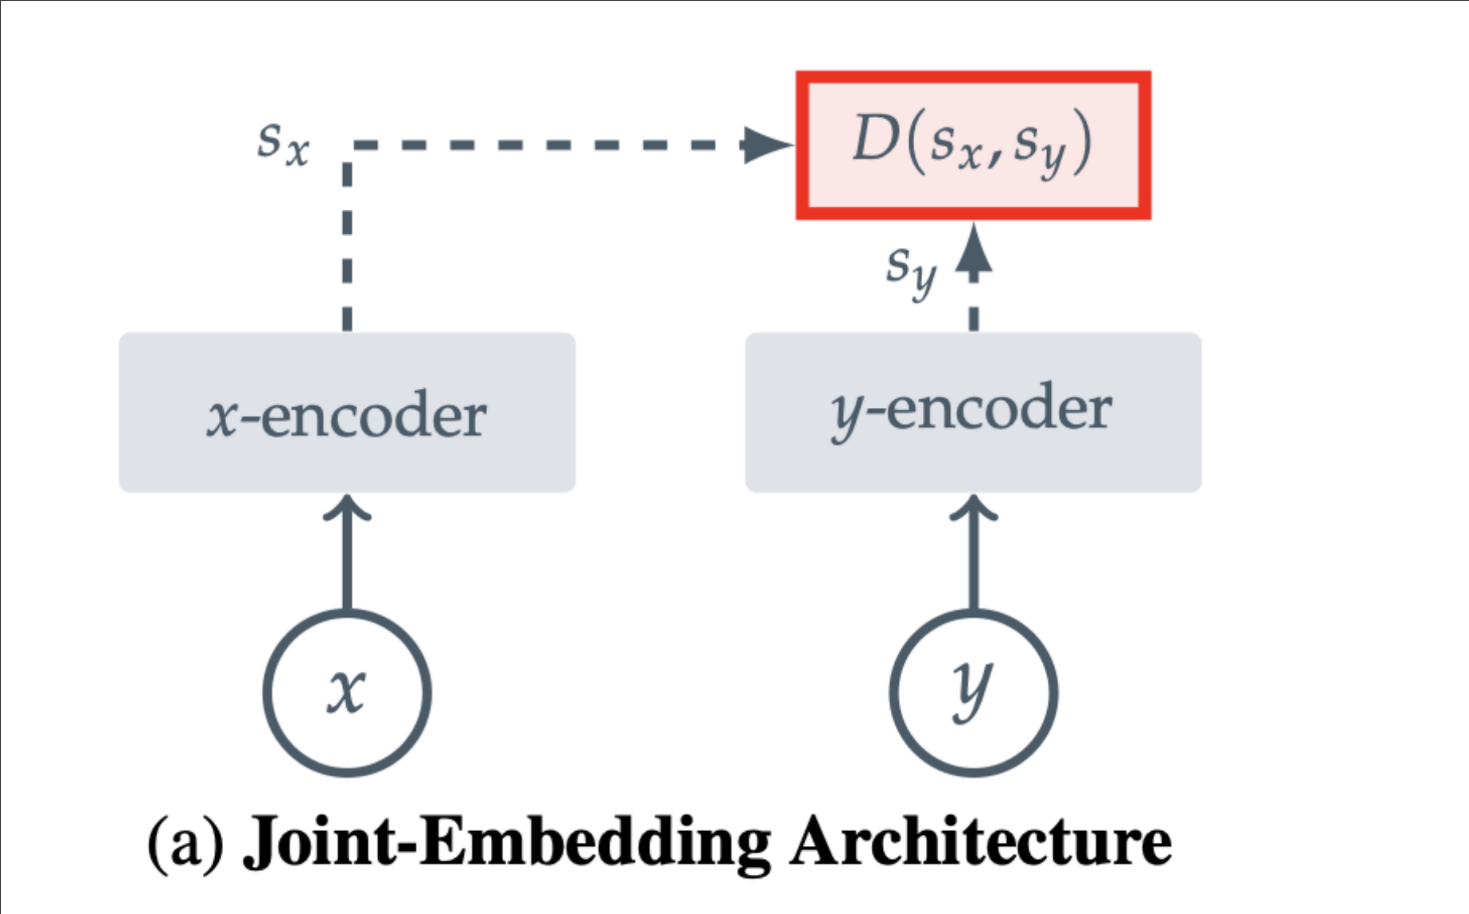
\includegraphics[width=0.4\textwidth]{clr.png}
\end{figure}

\end{frame}

\begin{frame}{Background}{Motivations for JEPA}
  \textbf{Generative Methods:}
  \begin{footnotesize}
This idea is at the core of self-supervised generative methods, which remove
or corrupt portions of the input and learn to predict the corrupted content.
In particular, mask-denoising approaches learn representations by reconstructing
randomly masked patches from an input, either at the pixel or token level.

Masked pretraining tasks require less
prior knowledge than view-invariance approaches and eas-
ily generalize beyond the image modality.

Only problem here is that they tend to underperform because
they build only lower level semantic relationships between jet-representations.

\end{footnotesize}
\begin{figure}
  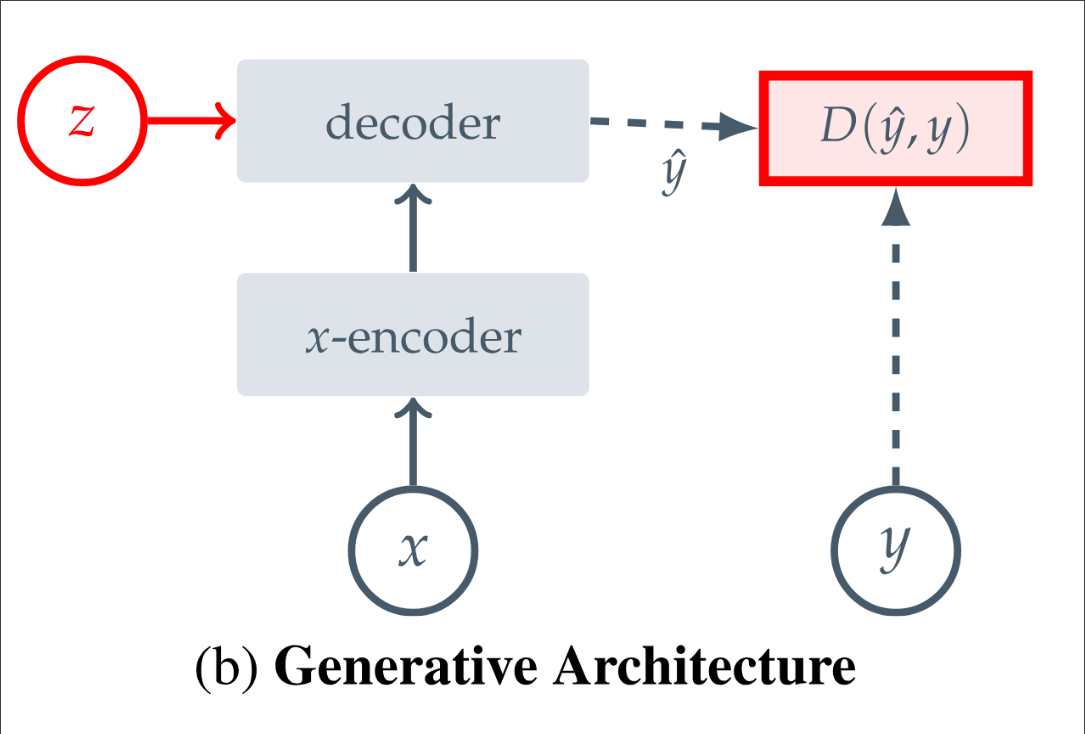
\includegraphics[width=0.4\textwidth]{gen.png}
\end{figure}

\end{frame}

\section{Architecture}
\begin{frame}{Architecutre}{JEPA}

\begin{figure}
  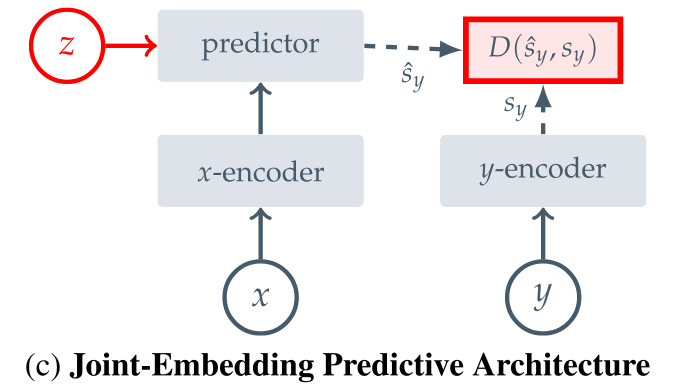
\includegraphics[width=0.4\textwidth]{jepa.png}
\end{figure}

Given a jet, we recluster it into subjets, masking some
as “target” subjets and defining others as “context” subjets. Then, we train a model to predict the
representations of target subjets based on the representations of context subjets, using the positions of
the target subjets as joint information.

This is also called Weakly-supervised model since the prediction stage uses some representations like
positions of the target subjects and help the prediction.

\end{frame}

\begin{frame}{Architecture}{J-JEPA}

\begin{figure}
  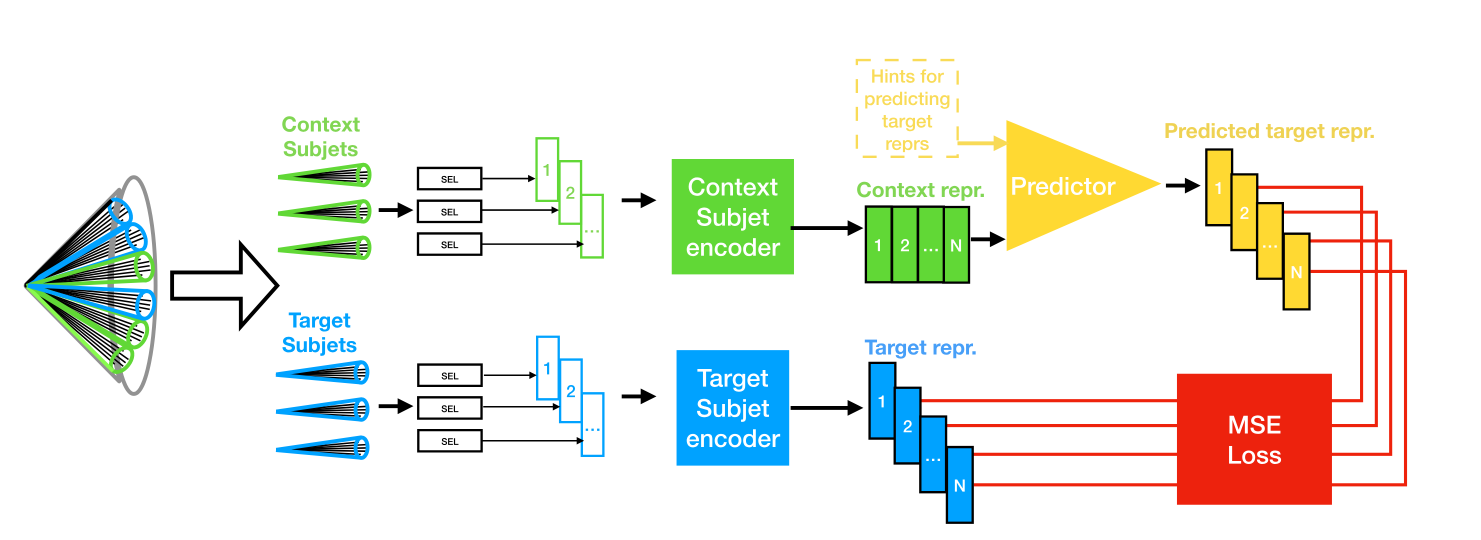
\includegraphics[width=0.7\textwidth]{jjepa.png}

  \begin{footnotesize}
    \begin{itemize}
      \item The J-JEPA architecture begins by splitting the large-radius jet (large black cone) into
target subjets and context subjets.

\item The context encoder and target encoder then separately generate
representations for the context subjets and the target subjets

\item  Using the positions of the target subjets
 as additional information (hints), the predictor takes the context representations and predicts the
 representations of the target subjets.

\item Finally, the L2 loss function is used to compare the predicted
 target subjet representations with the encoded target subjet representations, minimizing the difference
 between them
\end{itemize}
\end{footnotesize}
\end{figure}

\end{frame}

\section{Datasets and Training}
\begin{frame}{Datasets and Training}

\textbf{Datasets:}
\vspace{1em}

  \textbf{Pretraining:} JetClass: The pretraining task uses 1 Million jets, which is 1\% of Jetclass dataset.
It consists of 500k Top jets and 500k QCD jets.

\textbf{Finetuning:}
  TopTagging Reference Dataset:
      There are two scenarios in fine-tuning in this model. Both of
      them use TopTagging Dataset. The full dataset consists for 1.2 M Top jets.

      Another scenario is using 10\% of TopTagging dataset (120k jets). This is to
      represent situations where labeled training samplesare limited.

\vspace{2em}
\textbf{Training:}
 Experiments were performed on a single NVIDIA A100 GPU. For
 \begin{itemize}
   \item AdamW optimizer with cosine decay
   \item learning rate of $10^{-3}$, and weight decay $10^{-2}$
   \item Epochs: 80, batch-size: 64
 \end{itemize}

\end{frame}

\section{Evaluation}

\begin{frame}{Evaluation}
\textbf{Metrics:}

\begin{itemize}
  \item Compare finetuned model, with model trained from scratch (no pretraining).
  \item Prediction Accuracy (number of correct classifications vs wrong)
  \item Background rejection at signal efficiency 50\%.
\end{itemize}


\textbf{Other Evaluations:}

\begin{itemize}
  \item Using Traditional Embeddings vs. Custom Attension based embeddings
  \item Flattened subjets vs. Using class attention blocks to aggregate subject representations.
\end{itemize}

\end{frame}

\section{Results}

\begin{frame}{Results}
  \begin{figure}
    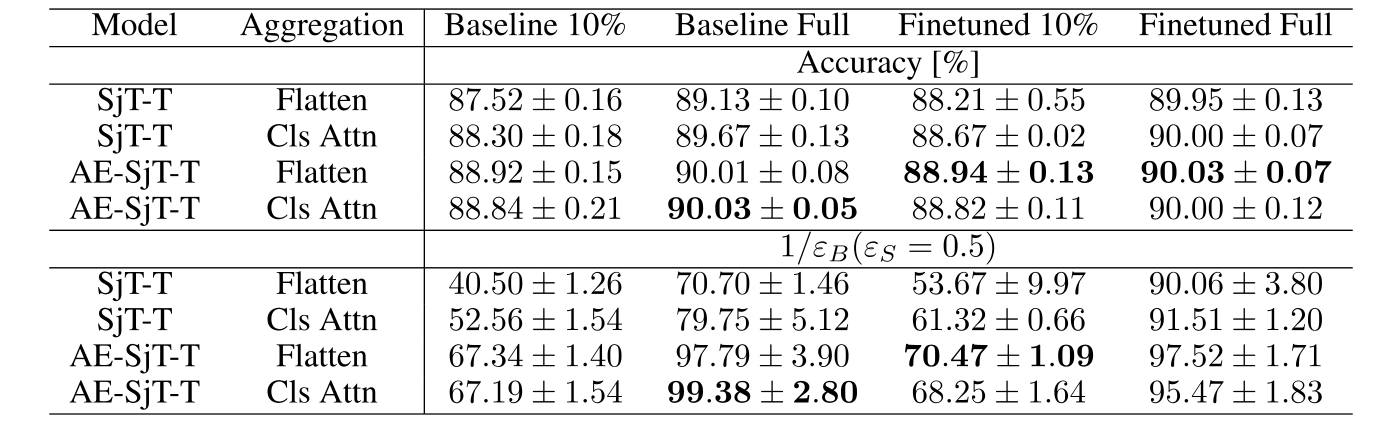
\includegraphics[width=0.9\textwidth]{results.png}
  \end{figure}

  \begin{figure}
    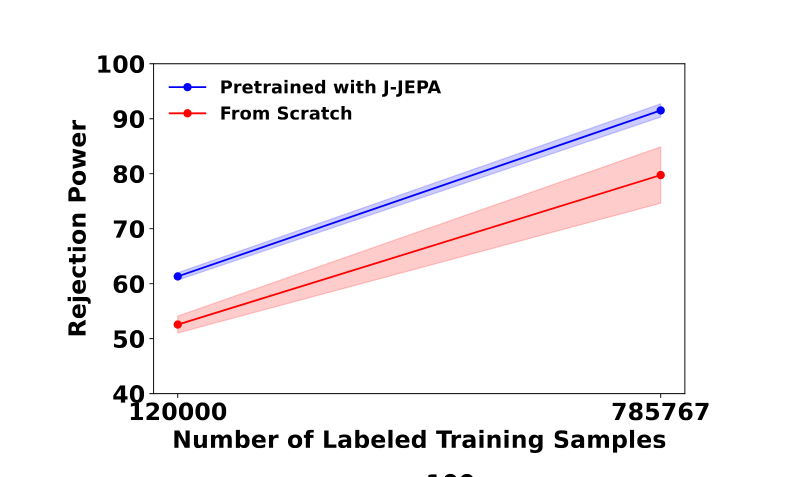
\includegraphics[width=0.5\textwidth]{results2.png}
  \end{figure}
\end{frame}

\section{Conclusion}

\begin{frame}{Conclusion}
This paper will likely have a follow-up which scales the data up
and uses different encoders and uses various different datasets.

The future work involves:
\begin{itemize}
  \item Implementing physics-informed architectures for the context
    and target encoders, such as the Particle Transformer
  \item Alternative strategies for embedding
    and defining targets and context
  \item Generalize the JEPA scheme to different physics objects: particles, events,
    detector readout, etc.
\end{itemize}

\end{frame}


\AtBeginSection[]{
  \begin{frame}
  \vfill
  \centering
  \begin{beamercolorbox}[sep=8pt,center,shadow=false,rounded=true]{title}
    \usebeamerfont{title}\huge \insertsectionhead\par%
  \end{beamercolorbox}
  \vfill
  \end{frame}
}

\begin{frame}
  \begin{beamercolorbox}[sep=8pt,center,shadow=false,rounded=true]{title}
  \centering \Huge
  Thank You
  \end{beamercolorbox}
\end{frame}


\end{document}
